\chapter{Project Planning and Design}

This chapter will outline the project planning and system design process, which will include discussions on the chosen project management methodology, the system architecture, the tech stack that will be used during development and the user interface design illustrated by using wireframes.

\section{UML Diagrams}

UML, or Unified Modeling Language, is a standardised modeling language that consists of a set of diagrams used for documenting software systems \parencite{uml}. It enables better communication potential of designs and architectural decisions. Common UML diagram types include:

\begin{itemize}
    \item \textbf{Use Case Diagram} --- Illustrates the system's intended functionality in terms of actors, use cases, and their relationships. It can be accompanied by a use case specifications document, which provides a description of each use case.
    \item \textbf{Sequence Diagram} --- Demonstrates how objects interact in a particular, timed sequence scenario, focusing on the messages passed between objects.
    \item \textbf{Activity Diagram} --- Represents the workflow of a target use case or business process through a series of activities, emphasizing steps, choices, iterations, and concurrency.
\end{itemize}

These diagrams were used to present the stakeholders with a visual representation of the system's design and functionalities. They can be found below, under their respective sub-sections.

\clearpage

\subsection{Use Case Diagram}
\begin{figure}[htbp]
    \centering
    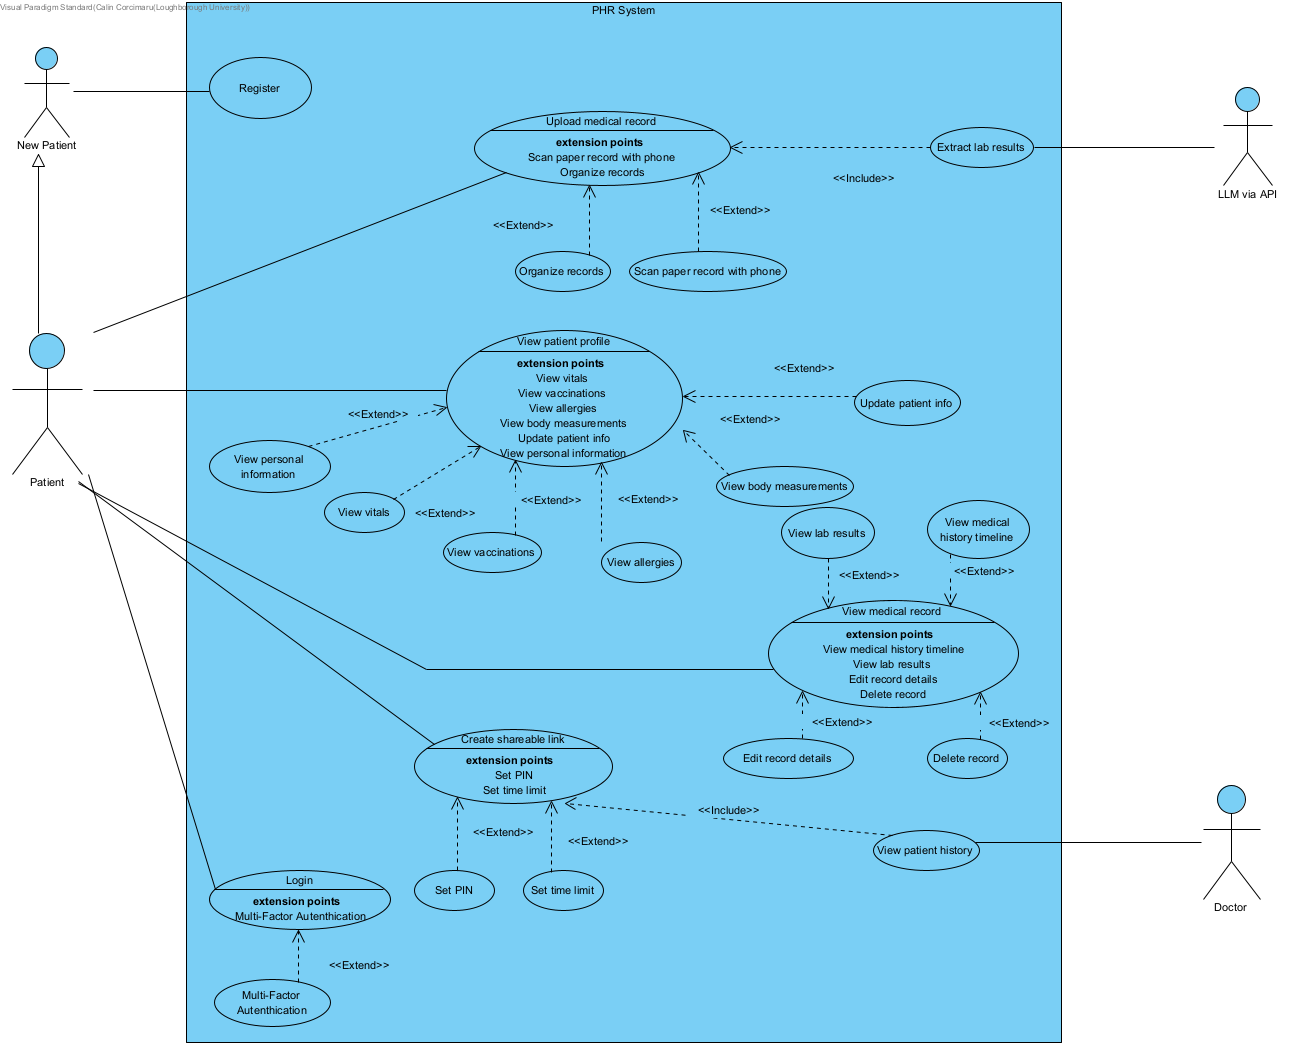
\includegraphics[width=\textwidth,height=0.7\textheight,keepaspectratio]{Use_Case.png}
    \caption{UML Use Case Diagram}\label{fig:uml_usecase}
\end{figure}

\FloatBarrier{}

\subsection{Use Case Specifications}

\subsubsection{Login}
\begin{tabular}{|p{0.2\textwidth}|p{0.7\textwidth}|}
\hline
Description & The Login use case allows the app user to log in to their existing account via their credentials, with an optional use of MFA. \\
\hline
Actors & Patient \\
\hline
Preconditions & Must have an existing account \\
\hline
Steps & 1. User enters user and password \newline
       2. User clicks on the login button \newline
       3. App validates user credentials \newline
       4. Patient enters MFA code if enabled \newline
       5. App logs user in \\
\hline
\end{tabular}

\subsubsection{Register}
\begin{tabular}{|p{0.2\textwidth}|p{0.7\textwidth}|}
\hline
Description & The Register use case allows the app user to create a new account. \\
\hline
Actors & New Patient \\
\hline
Preconditions & No existing account with the email used to register \\
\hline
Steps & 1. User enters user and password \newline
       2. User clicks on the register button \newline
       3. App validates user credentials \newline
       4. App logs user in \newline
       5. App sends verification email \newline
       6. User verifies email \\
\hline
\end{tabular}

\subsubsection{Upload Record}
\begin{tabular}{|p{0.2\textwidth}|p{0.7\textwidth}|}
\hline
Description & The Upload Record use case allows the patient to upload their medical records to the app. \\
\hline
Actors & Patient, LLM \\
\hline
Preconditions & Must be logged in \\
\hline
Steps & 1. User selects file upload (or camera scan) \newline
       2. User selects the record to upload \newline
       3. User clicks on the upload button \newline
       4. App validates the record \newline
       5. User selects the appropriate record type \newline
       6. If record type is lab result, app sends the record to LLM via API for processing into JSON format \newline
       7. App adds the record to the database \newline
       8. App shows confirmation to user \\
\hline
\end{tabular}

\subsubsection{Share Records}
\begin{tabular}{|p{0.2\textwidth}|p{0.7\textwidth}|}
\hline
Description & The Share Records use case allows the patient to share their medical records with doctors. \\
\hline
Actors & Patient, Doctor \\
\hline
Preconditions & Must be logged in and have records uploaded \\
\hline
Steps & 1. User selects option to create a share link \newline
       2. OPTIONAL\@: User selects the records to share \newline
       3. OPTIONAL\@: User adds a PIN to the share link \newline
       4. User selects time limit for the share link \newline
       5. App generates the share link \newline
       6. App sends the share link to the doctor via email \newline
       7. App shows confirmation to user \newline
       8. Doctor clicks on the share link \newline
       9. Doctor enters the PIN (if required) \newline
       10. App validates the PIN \newline
       11. App shows the records to the doctor \\
\hline
\end{tabular}

\subsubsection{View Records}
\begin{tabular}{|p{0.2\textwidth}|p{0.7\textwidth}|}
\hline
Description & The View Records use case allows the patient to view and edit their uploaded medical records. \\
\hline
Actors & Patient \\
\hline
Preconditions & Must be logged in and have records uploaded \\
\hline
Steps & 1. App provides a list of records or medical history \newline
       2. User selects record to view from list or medical history \newline
       3. App retrieves the record from the database \newline
       4. App shows the record to the user \newline
       5. OPTIONAL\@: User can view the record in a graphical format if lab result \newline
       6. OPTIONAL\@: User edits the record \newline
       7. OPTIONAL\@: User deletes the record \\
\hline
\end{tabular}

\subsubsection{View Patient Profile}
\begin{tabular}{|p{0.2\textwidth}|p{0.7\textwidth}|}
\hline
Description & The View Patient Profile use case allows the patient to view and edit their profile information, including health information such as allergies, medications, vaccinations and recorded health data like blood pressure, glucose levels, etc. \\
\hline
Actors & Patient \\
\hline
Preconditions & Must be logged in \\
\hline
Steps & 1. User selects the profile section \newline
       2. App retrieves the profile information from the database \newline
       3. App shows the profile information to the user --- vaccinations, allergies, medications, health data \newline
       4. OPTIONAL\@: User edits the profile information \newline
       5. OPTIONAL\@: User adds new health data \newline
       6. OPTIONAL\@: User deletes health data \newline
       7. OPTIONAL\@: User can view health data in a graphical format \\
\hline
\end{tabular}

\FloatBarrier{}
\clearpage

\subsection{Sequence Diagrams}
\begin{figure}[htbp]
    \centering
    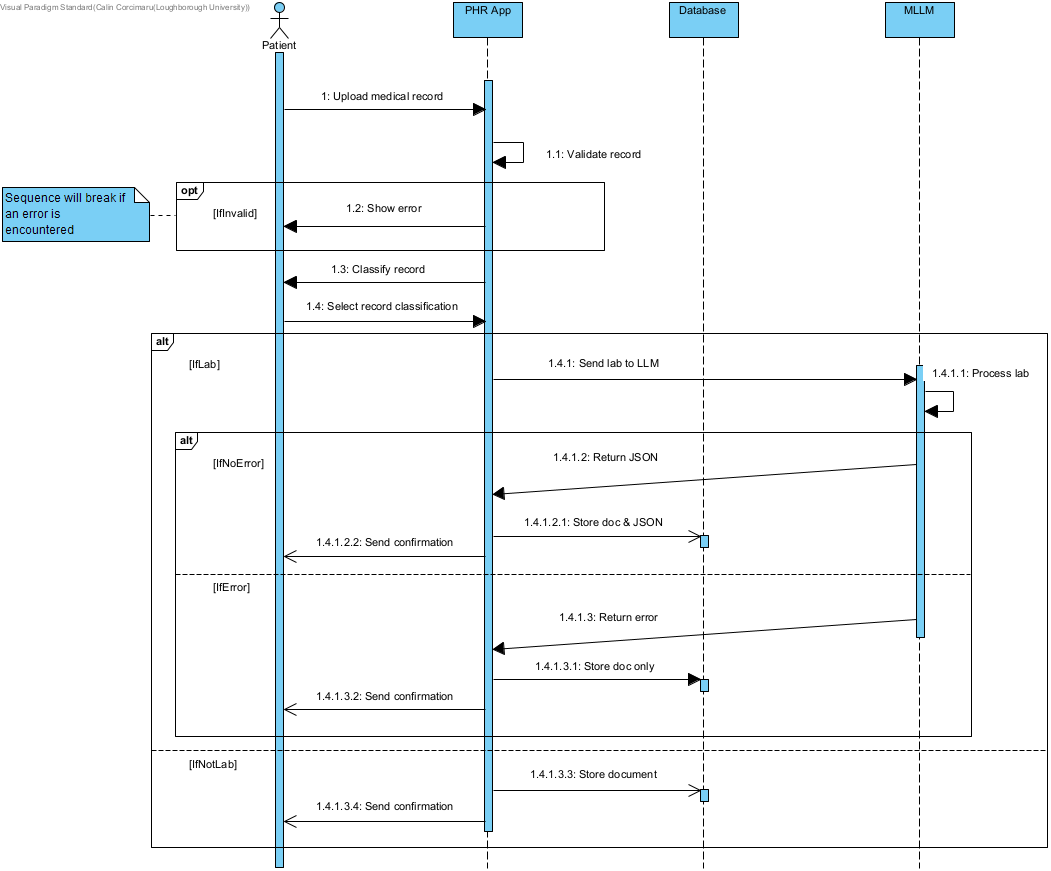
\includegraphics[width=\textwidth,height=0.8\textheight,keepaspectratio]{Sequence_upload.png}
    \caption{UML Sequence Diagram --- Upload Record Use Case}\label{fig:sequence1}
\end{figure}

\begin{figure}[htbp]
    \centering
    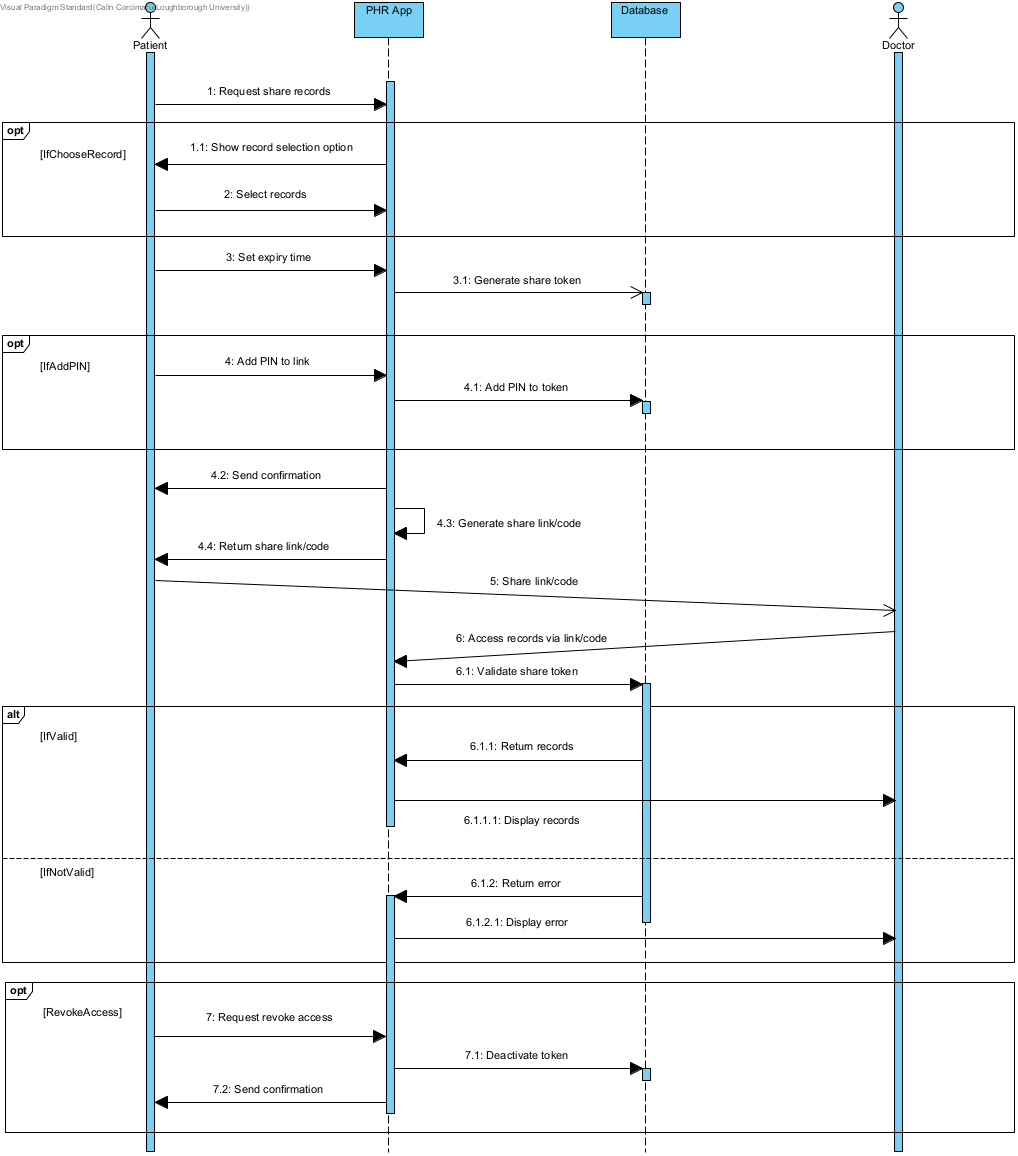
\includegraphics[width=\textwidth,height=0.8\textheight,keepaspectratio]{Sequence_share.png}
    \caption{UML Sequence Diagram --- Share Records Use Case}\label{fig:sequence2}
\end{figure}

\FloatBarrier{}

\noindent\begin{minipage}{\textwidth}
    \subsection{Activity Diagrams}
    \begin{center}
        \rotatebox[origin=c]{270}{
            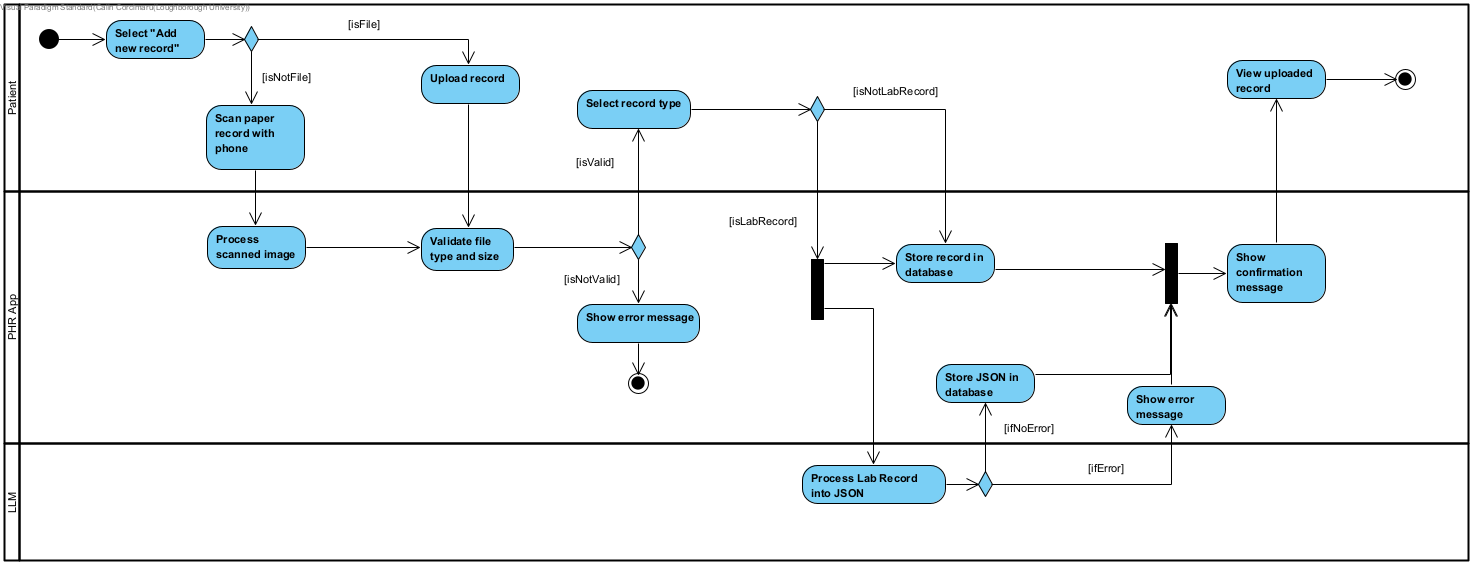
\includegraphics[width=0.9\textheight,keepaspectratio]{Activity_upload.png}
        }
        \captionof{figure}{UML Activity Diagram - Upload Record Use Case}\label{fig:activity1}
    \end{center}
\end{minipage}

\noindent\begin{minipage}{\textwidth}
    \begin{center}
        \rotatebox[origin=c]{270}{
            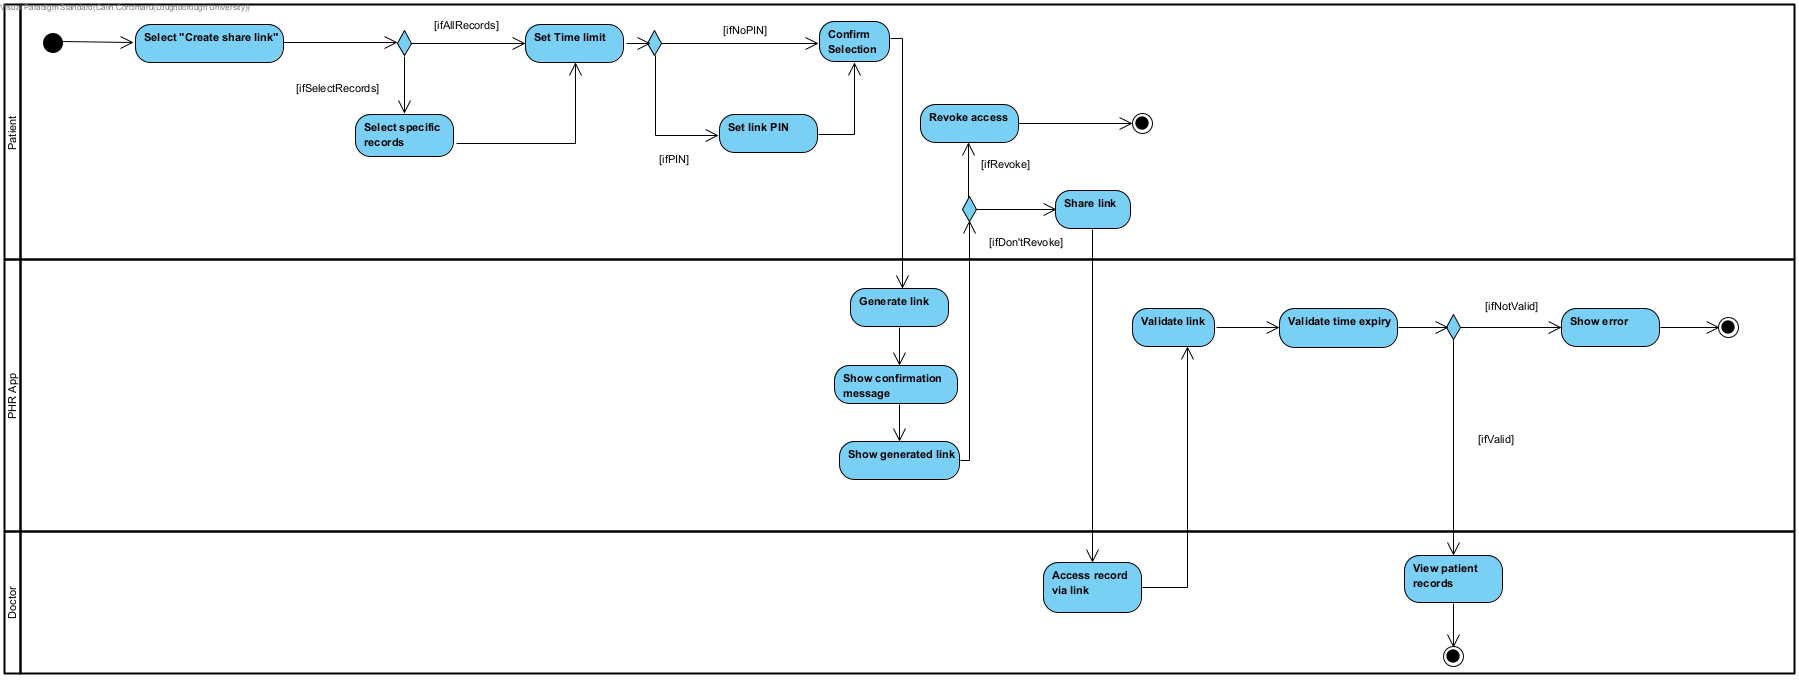
\includegraphics[width=0.9\textheight,keepaspectratio]{Activity_link.png}
        }
        \captionof{figure}{UML Activity Diagram - Share Records Use Case}\label{fig:activity2}
    \end{center}
\end{minipage}

\FloatBarrier{}

\noindent\begin{minipage}{\textwidth}
    \section{Database Design}
    \begin{center}
        \rotatebox[origin=c]{270}{
            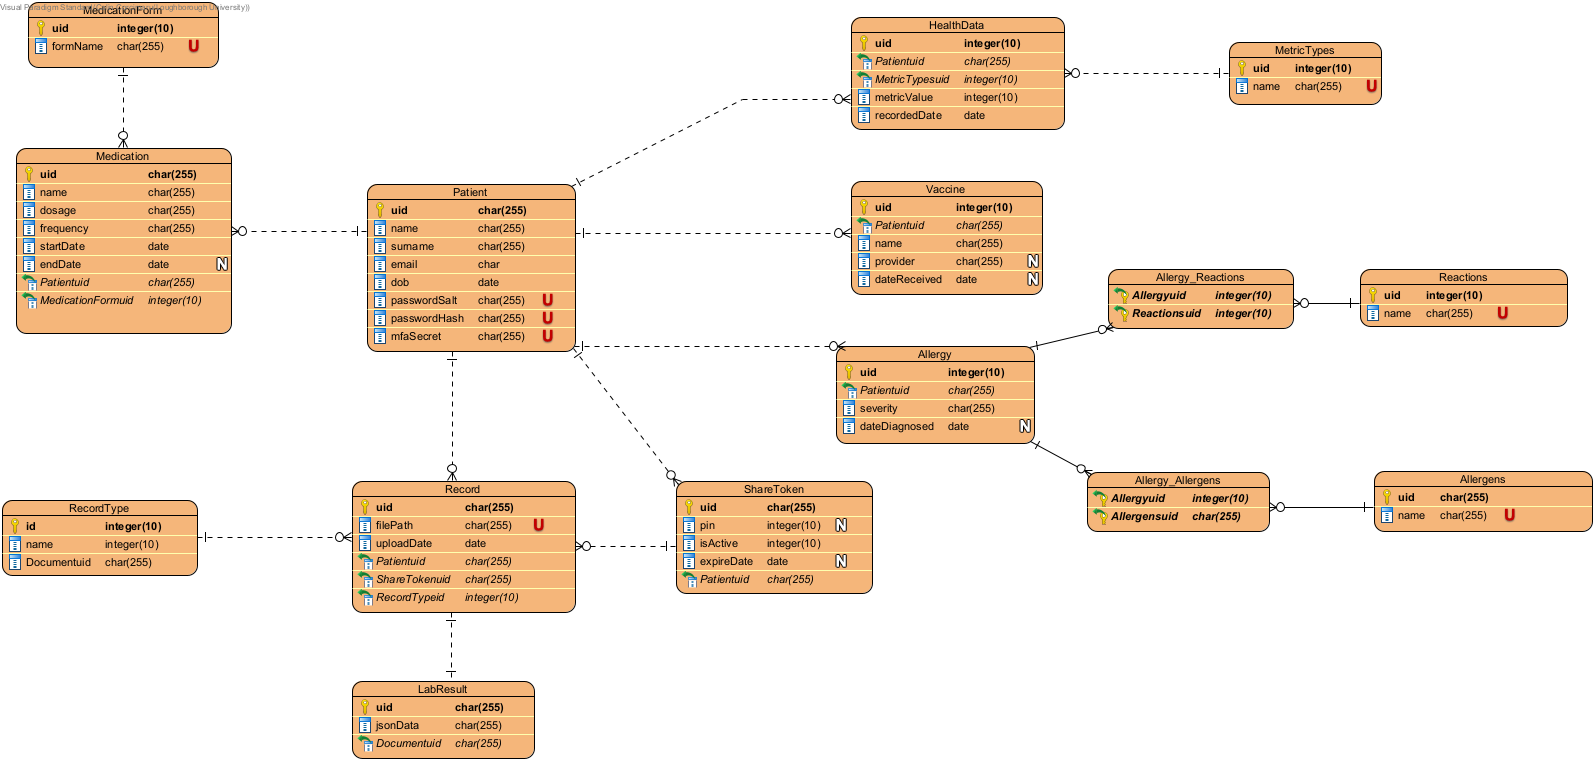
\includegraphics[width=0.9\textheight,keepaspectratio]{ERD.png}
        }
        \captionof{figure}{Entity Relationship Diagram}\label{fig:erd}
    \end{center}
\end{minipage}

\FloatBarrier{}

\section{Wireframes}

Wireframes were used to provide a high-level overview of the application's design and present some of its key functionalities. These have been created using Figma and presented to key stakeholders during virtual meetings. Based on the feedback received, the wireframes have been adjusted and some examples can be seen in figures~\ref{fig:dashboard},~\ref{fig:medhistory} and~\ref{fig:lab}. The full set of wireframes can be found in appendix~\ref{sec:wireframes}.

\begin{figure}[ht]
    \centering
    \begin{minipage}[c]{0.70\textwidth}
        \subfloat[Desktop version]{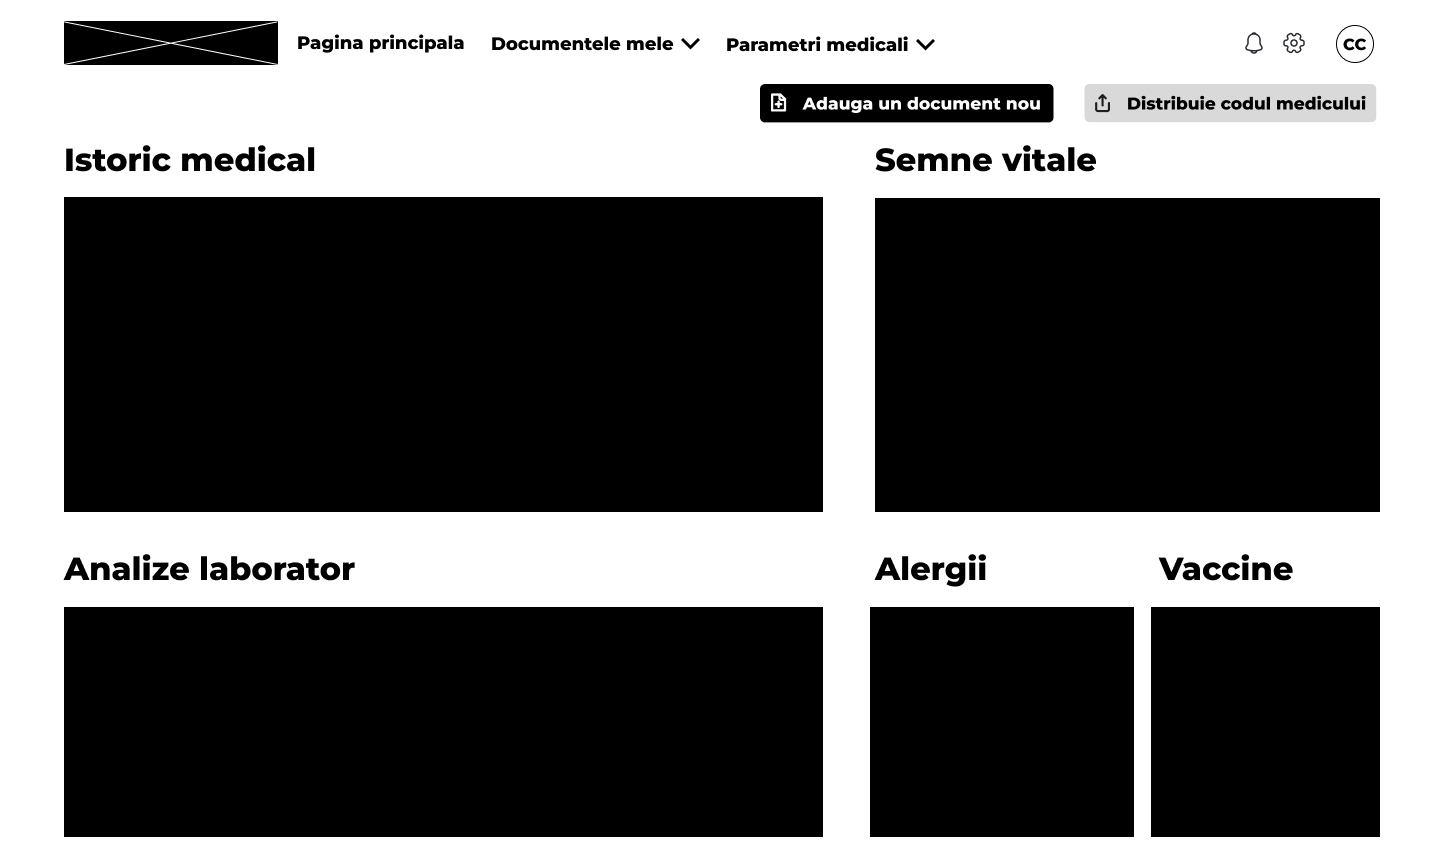
\includegraphics[width=\textwidth]{wireframes/Desktop_dashboard.png}\label{fig:dashboard-desktop}}
    \end{minipage}
    \hspace{0.05\textwidth}
    \begin{minipage}[c]{0.20\textwidth}
        \subfloat[Mobile version]{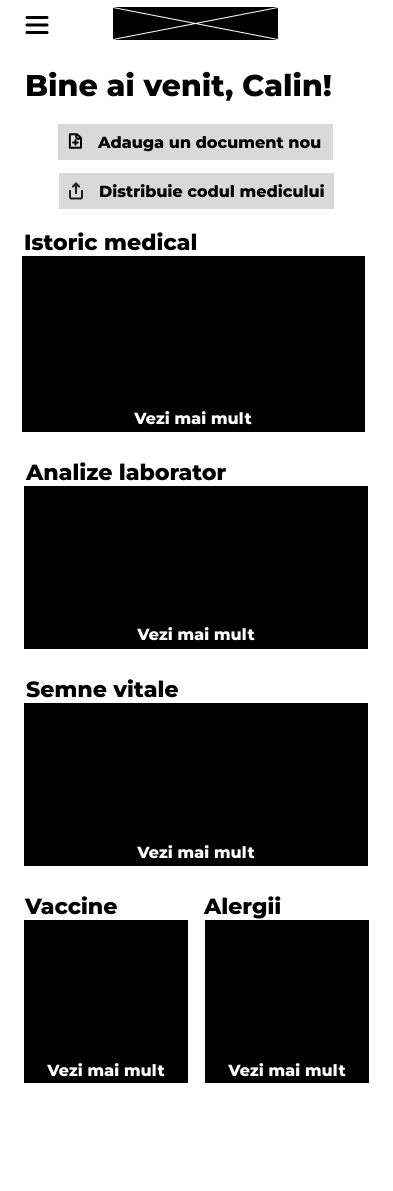
\includegraphics[width=\textwidth]{wireframes/Mobile_dashboard.png}\label{fig:dashboard-mobile}}
    \end{minipage}
    \caption{Desktop and Mobile version of the Dashboard screen}\label{fig:dashboard}
\end{figure}

\begin{figure}[ht]
    \centering
    \begin{minipage}[c]{0.70\textwidth}
        \subfloat[Desktop version]{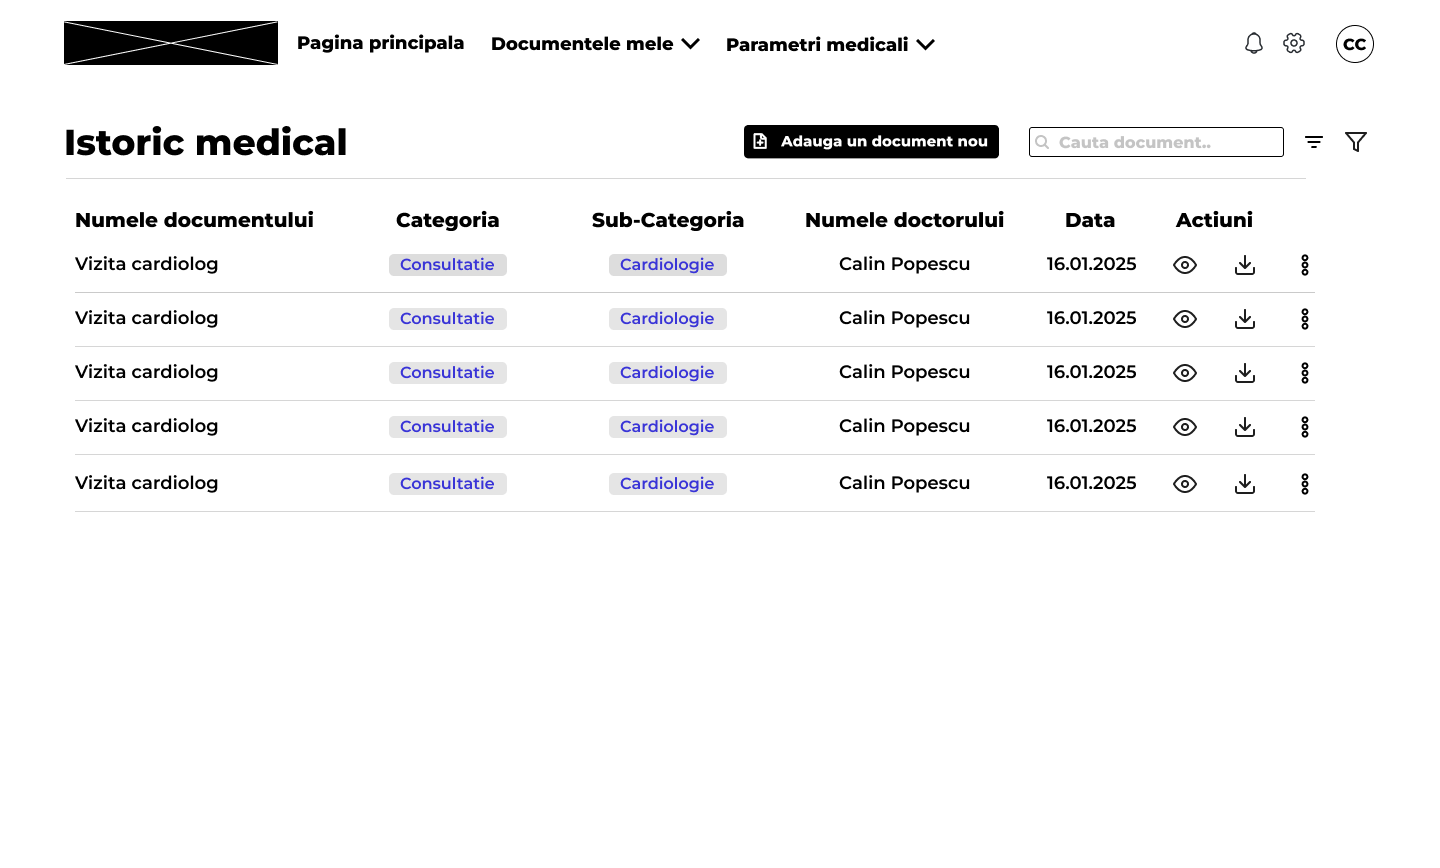
\includegraphics[width=\textwidth]{wireframes/Desktop_medHistory.png}\label{fig:medhistory-desktop}}
    \end{minipage}
    \hspace{0.05\textwidth}
    \begin{minipage}[c]{0.20\textwidth}
        \subfloat[Mobile version]{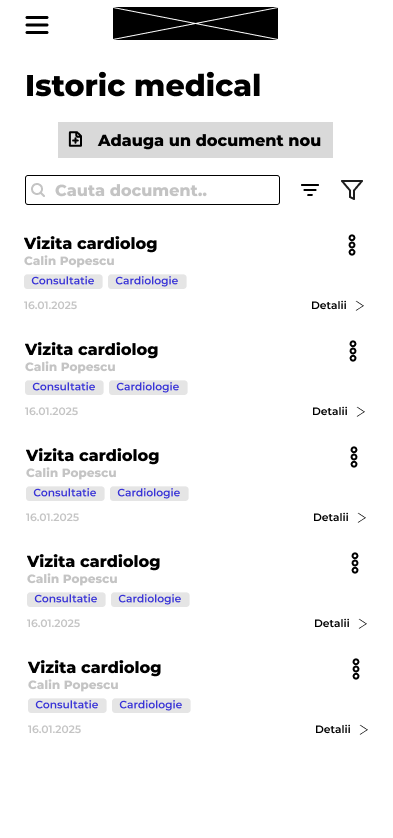
\includegraphics[width=\textwidth]{wireframes/Mobile_medHistory.png}\label{fig:medhistory-mobile}}
    \end{minipage}
    \caption{Desktop and Mobile version of the Medical History screen}\label{fig:medhistory}
\end{figure}

\begin{figure}[ht]
    \centering
    \begin{minipage}[c]{0.70\textwidth}
        \subfloat[Desktop version]{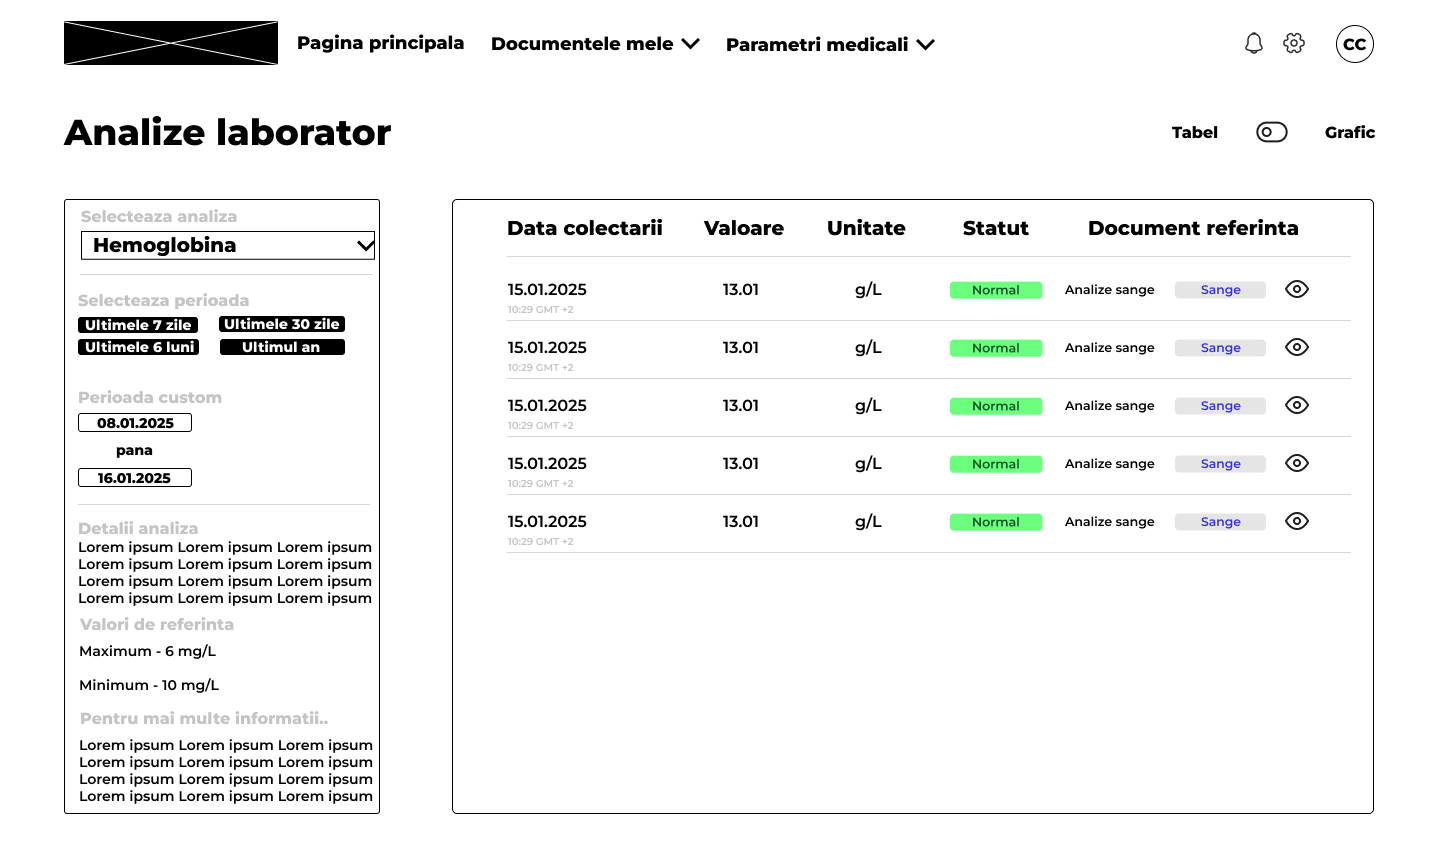
\includegraphics[width=\textwidth]{wireframes/Desktop_labTest.png}\label{fig:lab-desktop}}
    \end{minipage}
    \hspace{0.05\textwidth}
    \begin{minipage}[c]{0.20\textwidth}
        \subfloat[Mobile version]{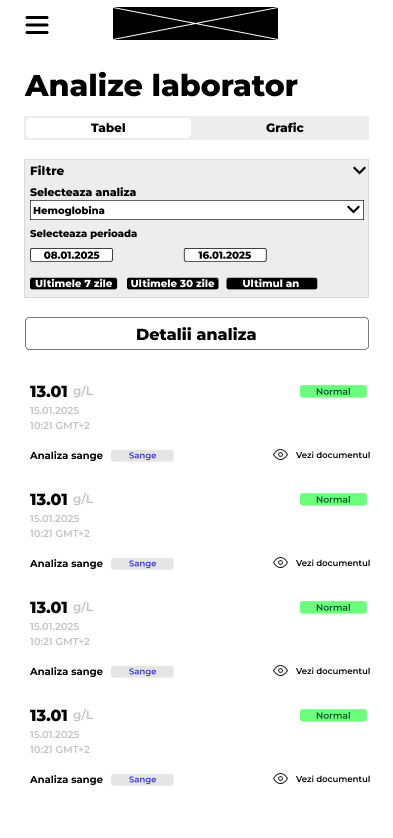
\includegraphics[width=\textwidth]{wireframes/Mobile_labTest.png}\label{fig:lab-mobile}}
    \end{minipage}
    \caption{Desktop and Mobile version of the Lab Test Results screen}\label{fig:lab}
\end{figure}

\section{Project Tech Stack}\label{sec:techstack}

Based on the research conducted in sections~\ref{sec:database},~\ref{sec:backend} and~\ref{sec:frontend}, the following tech stack was chosen for the project, which can be seen in diagram~\ref{fig:architecture}.

\begin{figure}[htbp]
    \centering
    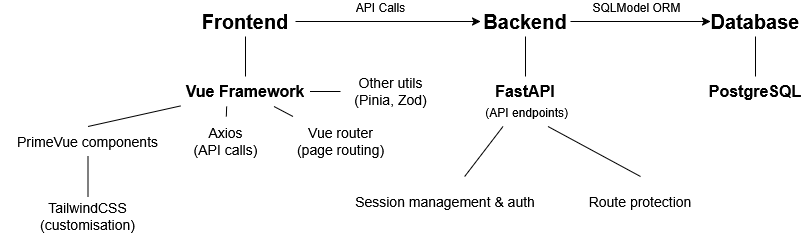
\includegraphics[width=0.8\textwidth]{Sytem_architecture.png}
    \caption{Proposed System Architecture}\label{fig:architecture}
\end{figure}

\subsection{Frontend}

Vue was chosen for the frontend, as it is a JavaScript framework used for building single-page applications (SPAs) known for its ease of use and flexibility \parencite{vue}. It is powered by components, element reactivity and Single File Components (SFCs) that enable HTML, CSS and JS to be used in a single \lstinline{.vue} file. Vue also boasts a large and active community, with many libraries and guides available for developers. Previous experience with Vue made it a suitable choice for this project. Diagram~\ref{fig:frontend} showcases how different elements of the frontend interact. The next subsections will briefly discuss each.

\begin{figure}[htbp]
    \centering
    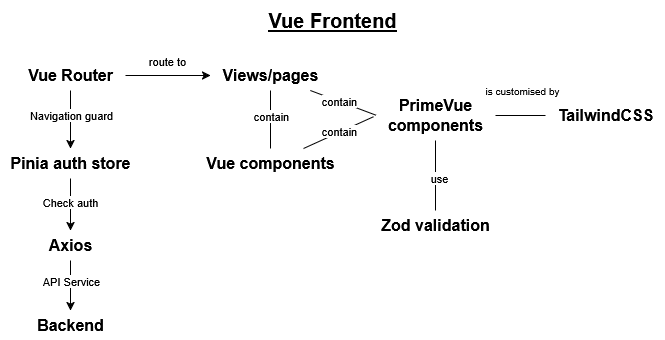
\includegraphics[width=0.8\textwidth]{frontend.png}
    \caption{Interaction of Frontend Components}\label{fig:frontend}
\end{figure}

\FloatBarrier{}
\subsubsection{Vue Router}

Vue Router is the official client-side router for Vue.js, which allows the user to navigate between application pages without a full reload \parencite{vuerouter}. It makes full use of the SPA capabilities of Vue, providing a seamless user experience. Vue Router can also be used to create navigation guards to protect certain routes from unauthorized access, which is crucial for the security of the application.

\subsubsection{Pinia}

Pinia is a store library for Vue made by the same team \parencite{pinia}. Its main functionality is to provide a way to share states across Vue components and pages. In this project, Pinia will be used to store the user's authentication status and other global states that need to be shared within the application.

\subsubsection{Axios}

Axios is a promise-based HTTP client for the browser and Node.js \parencite{axios}. It is used to make HTTP requests to the backend. Similarly, it allows for automatic interaction with cookies in requests and responses, which is important for API communication.

\subsubsection{Vue views and components}

Vue components and views are the foundation of the frontend. Views represent the different pages of the application, which can be navigated to using the Vue Router. Components allow to break down the UI into independent and reusable elements \parencite{vuecomponents}. Each component can be stored in a separate \lstinline{.vue} file and imported when necessary.

\subsubsection{PrimeVue and TailwindCSS}

PrimeVue is a component library for Vue, which provides a set of pre-built components that can be used to easily create the frontend of the application \parencite{primevue}. TailwindCSS is a CSS framework that provides a multitude of classes that can be applied to style application elements \parencite{tailwind}. When combined, PrimeVue provides the basic building blocks such as buttons, forms, and tables, while TailwindCSS styles these components.

\subsection{Backend}

FastAPI was chosen as the backend framework. It is a modern framework used in building APIs with Python, chosen due to its ease of use, simplicity and heaps of documentation available \parencite{fastapi}. Previous experience with Python made this framework an accessible choice for this project. A separate backend would also allow for future flexibility --- its independence from the frontend enables it to be re-used for other platforms, such as mobile. Diagram~\ref{fig:backend} shows how different components of the backend will interact with each other.

\begin{figure}[htbp]
    \centering
    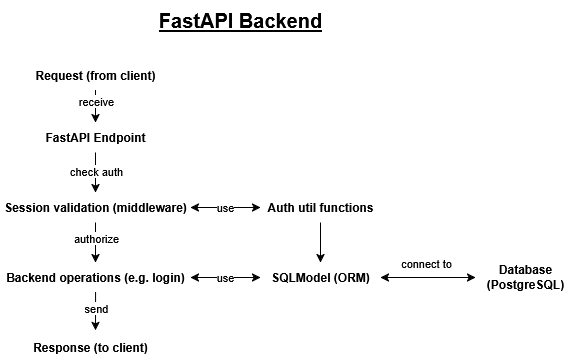
\includegraphics[width=\textwidth,height=0.8\textheight,keepaspectratio]{backend.png}
    \caption{Interaction of Backend Components}\label{fig:backend}
\end{figure}

\FloatBarrier{}

\subsection{Database}

PostgreSQL was the database of choice, which is a relational database system that boasts a good reputation for its reliability, wide feature set and performance \parencite{postgres}. It supports a wide range of data types, including JSON and UUID, which are important for this project. Similarly, PostgreSQL offers robust security features like an access-control system or column and row-level security. 

SQLModel, a Python library built on top of SQLAlchemy and Pydantic, will be used to interact with the database. SQLModel provides a way to define database tables using classes, which are then used to interact with the database \parencite{sqlmodel}.

\section{Project Management}

\subsection{Methodology and Tools}

Based on the research in section~\ref{sec:methodologies}, a hybrid project management approach has been adopted, with Waterfall as the main methodology covering the initial phases of the project that transitions to Agile during the development phase.

\begin{enumerate}
    \item \textbf{The nature of the project:} The limited timeframe and resources required using a flexible approach to ensure a viable prototype is delivered.
    \item \textbf{Documentation requirements:} The academic nature of this project calls for extensive documentation of requirements, design choices and implementation decisions. 
    \item \textbf{Stakeholder engagement:} The development will require continuous stakeholder feedback to ensure the solution meets stakeholder needs.
\end{enumerate}

Notion will be used as the project management tool. It allows for easy task management and documentation, providing a wide range of templates for Gantt charts, user stories, backlogs, sprints and Kanban boards \parencite{notion}. 

\subsection{Sprint planning}

Following the completion of the initial project phases, the development phase will be divided into 6 sprints. Each sprint will last 2 weeks, with a total of 12 weeks allocated. The sprints will be planned as follows:

\begin{itemize}
    \item \textbf{Sprint 1} --- Will configure the development environment, frameworks, database and implement core functionalities like user authentication and registration.
    \item \textbf{Sprint 2} --- Will implement the vaccines, allergies, medications and health data sections alongside the a basic layout of the dashboard.
    \item \textbf{Sprint 3} --- Will complete the main dashboard and implement the document upload feature alongside the medical history section.
    \item \textbf{Sprint 4} --- Will integrate the MLLM and implement the automated lab test extraction feature.
    \item \textbf{Sprint 5} --- Will develop the record sharing feature via a shareable link, as well as the doctor view of the records.
    \item \textbf{Sprint 6} --- Will address any identified remaining gaps, such as missing features, as well as final testing processes.
\end{itemize}
